\chapter{Related work}
This chapter explains the necessary basis to understand the procedure and contains all relevant information of previous work in this field.
\section{Basic machine learning algorithms}
%entry text

\subsection{Linear regression}
Linear regression is one of the earliest statistical models \autocite{freedman2009}. It assumes a linear dependency to estimate the value of a unit's dependent variable based on one or more of the unit's explanatory variables. A simple linear regression multiplies the dependent variable $x$ with the slope $\beta_1$ and adds the intercept $\beta_0$ to receive the estimated target value $\hat{y}$.
\begin{equation}
    \hat{y} = \beta_0 + \beta_1 x
\end{equation}

To use multiple explanatory variables $x_1, \ldots, x_p$, the same amount $p$ of regression coefficients $\beta_1, \ldots, \beta_p$ are needed.
\begin{equation}
    \hat{y} = \beta_0 + \beta_1 x_1 + \cdots + \beta_p x_p
\end{equation}

The coefficients and $\beta_0$ can be combined to the column vector $\boldsymbol{\beta}$ and analogous can the explanatory variables be combined to the row vector $\mathbf{x}$ using $1$ as first element.
\begin{equation}
    \boldsymbol{\beta} = \begin{bmatrix}\beta_0\\\beta_1\\\vdots\\\beta_p\end{bmatrix}\text{,}\quad
    \mathbf{x} = \begin{bmatrix}1&x_1&\cdots&x_p\end{bmatrix}
\end{equation}

This enables more compact notations such as the matrix notation.
\begin{equation}
    \hat{y} = \sum_{i=0}^p \beta_i x_i = \beta_0 x_0 + \beta_1 x_1 + \cdots + \beta_p x_p = \mathbf{x}\boldsymbol{\beta}
\end{equation}

The error variable $\epsilon$ represents the difference between the actual value $y$ of a unit and its estimation $\hat{y}$. It includes all factors not explained by a linear relationship. 
\begin{equation}
    \epsilon = y - \hat{y}
    % \text{,}\quad
    % y = \mathbf{x}\boldsymbol{\beta} + \epsilon
\end{equation}

$n$ units can be stacked using the matrix $\mathbf{X}$ for the explanatory variables and the column vector $\mathbf{\hat{y}}$ for the corresponding estimations. Additionally, the actual values $\mathbf{y}$ and the error variable $\boldsymbol{\epsilon}$ can be expressed the same way.
\begin{equation}
    \mathbf{X} = \begin{bmatrix}1&x_{1,1}&\cdots &x_{1,p}\\\vdots&\vdots&\ddots&\vdots\\1&x_{n,1}&\cdots &x_{n,p}\end{bmatrix}\text{,}\quad
    \mathbf{\hat{y}} = \begin{bmatrix}\hat{y}_1\\\vdots\\\hat{y}_n\end{bmatrix}\text{,}\quad
    \mathbf{y} = \begin{bmatrix}y_1\\\vdots\\y_n\end{bmatrix}\text{,}\quad
    \boldsymbol{\epsilon} = \begin{bmatrix}\epsilon_1\\\vdots\\\epsilon_n\end{bmatrix}
\end{equation}

This leaves the following notations for the model, estimation and error.
\begin{equation}
    \mathbf{y} = \mathbf{X}\boldsymbol{\beta} + \boldsymbol{\epsilon}\text{,}\quad
    \mathbf{\hat{y}} = \mathbf{X}\boldsymbol{\beta}\text{,}\quad
    \boldsymbol{\epsilon} = \mathbf{y} - \mathbf{\hat{y}} = \mathbf{y} - \mathbf{X}\boldsymbol{\beta}
\end{equation}

Loss functions calculate a value for the total error on a given data set. For regression problems the \gls{mse} is most commonly used. The squares prevent positive and negative deviations to cancel each other out, but outliers are weighted disproportionately. For data sets with many outliers it can make sense to choose another loss function. 
%The averaging allows the comparison of losses from different subsets
\begin{equation}
    \mathcal{L}_{MSE} = \frac{1}{n}\sum_{i=1}^{n} {(y_i - \hat{y_i})}^2 = \frac{1}{n}\sum_{i=1}^{n} {(\epsilon_i)}^2
\end{equation}

The loss $\mathcal{L}$ should be minimal for accurate estimations. In case of the \gls{mse} the optimal parameters $\boldsymbol{\hat{\beta}}$ could be calculated, provided $p < n$ and the $p$ columns of $\mathbf{X}$ are linearly independent.
\begin{equation}
    \boldsymbol{\hat{\beta}} = (\mathbf{X}^T\mathbf{X})^{-1}\mathbf{X}^{T}\mathbf{y}
\end{equation}
The computational complexity of this closed solution is nearly cubic $O(n^3)$ due to the calculating of the matrix inverse, making it unfeasible for almost all data sets \autocite{riahi2023}. Therefore   

A common way of \gls{ml} to find good parameters $\boldsymbol{\beta}$ is through gradient descent \autocite{robbins1951}. 
\gls{sgd} starts with randomly initialized values for $\boldsymbol{\theta}_0$ and a predefined learning rate $\alpha$. 
During every step $k$ the partial derivatives of the loss function $J(\boldsymbol{\theta}_k)$ with respect to the current parameters $\boldsymbol{\theta}_k$ get calculated. The parameters can then be updated and used in the next step.
\begin{equation}
    \boldsymbol{\theta}_{k+1} = \boldsymbol{\theta}_k - \alpha\nabla J(\boldsymbol{\theta}_k)\text{,}\quad k=0,1,2,\ldots
\end{equation}
This step is repeated until the result approaches an optimum and the progress negligible. Instead of using all the available data, it is common practise to separate the data into a training and validation subset. The latter can be used to track the performance of unseen data, which is crucial to prevent overfitting. While \gls{sgd} uses a single sample per iteration to update the parameters, batch gradient descent uses the average of all data points within the training set to update the parameters. Mini-batch gradient descent is an approach in between using a subset of training data every iteration. 

% Logistic Regression

% Using the \gls{mse} as loss function the partial derivatives can be calculated as follows.
% \begin{equation}
    % \nabla\mathcal{L}_{MSE} = \frac{\partial J(\boldsymbol{\theta}_k)}{\partial \boldsymbol{\theta}_k} = \frac{2}{n} \mathbf{X}^{T}(\mathbf{X}\boldsymbol{\theta}_k - \mathbf{X}^{T}\mathbf{y})
% \end{equation}

Libraries like ``scikit'' use algorithms like limited-memory BFGS to accelerate the calculations of linear models. For neural networks gradient descent based approaches have prevailed.

\subsection{k-nearest neighbors}
\gls{knn} is an algorithm for classification and regression using the $k$ closest training samples \autocite{fix1989,cover1967}. The feature vector and the according target value of every provided training sample is stored. The feature vectors of further samples can be compared with a distance metric to find similar training samples. Common metrics are the Euclidean distance or the Manhattan distance. The cosine similarity can also be used, where vector magnitude is not critical. 
The class labels of the $k$ nearest neighbors serve as basis for the output. For classification often a simple majority voting is done. It is also possible to use the distance to give more weight to closer samples.
The optimal $k$ is usually determined by calculating multiple values and comparing the resulting score. With a skewed dataset and simple majority voting, $k$ will most likely be relatively small, because many neighbors benefit large classes and therefore hinder the prediction of smaller classes.
% more content

\section{Basic artificial neural networks}
\subsection{Artificial neurons}
Artificial neurons were originally invented for binary classifications and mimic biological neurons \autocite{mcculloch1943}. Several input values are summed up and compared with a predefined threshold value to receive a binary output. This neuron was supplemented with weight values and a bias value to function as a linear regression, while the weights correspond to the slopes and the bias to the intercept  \autocite{rosenblatt1957}. This system can mathematically be described with a column vector $\mathbf{x}$ for the $n$ input, the scalar $b$ for the bias and the row vector $\mathbf{w}$ for the weight values.

\begin{equation}
    \text{$b \in \mathbb{R}$,}\quad\mathbf{w} = \begin{bmatrix}w_1&\cdots &w_n\end{bmatrix}\text{,}\quad\mathbf{x} = \begin{bmatrix}x_1\\\vdots \\x_n\end{bmatrix}\quad\text{for $\mathbf{w}$, $\mathbf{x} \in \mathbb{R}^n$}
\end{equation}

The summation results in the intermediate value $z$.

\begin{equation} \label{eq:z}
    z = \sum_{i=1}^n w_i x_i + b = \mathbf{w} \cdot \mathbf{x} + b
\end{equation}

An activation function $g$ is applied to $z$ to calculate the output $\hat{y}$.

\begin{equation} \label{eq:y}
\hat{y} = g(z) = g(\mathbf{w} \cdot \mathbf{x} + b)
\end{equation}

The Figure~\ref{fig:neuron} visualizes the mentioned procedure, while the steps \ref{eq:z} and \ref{eq:y} are combined within the neuron.

\begin{figure}[H]
    \begin{center}
    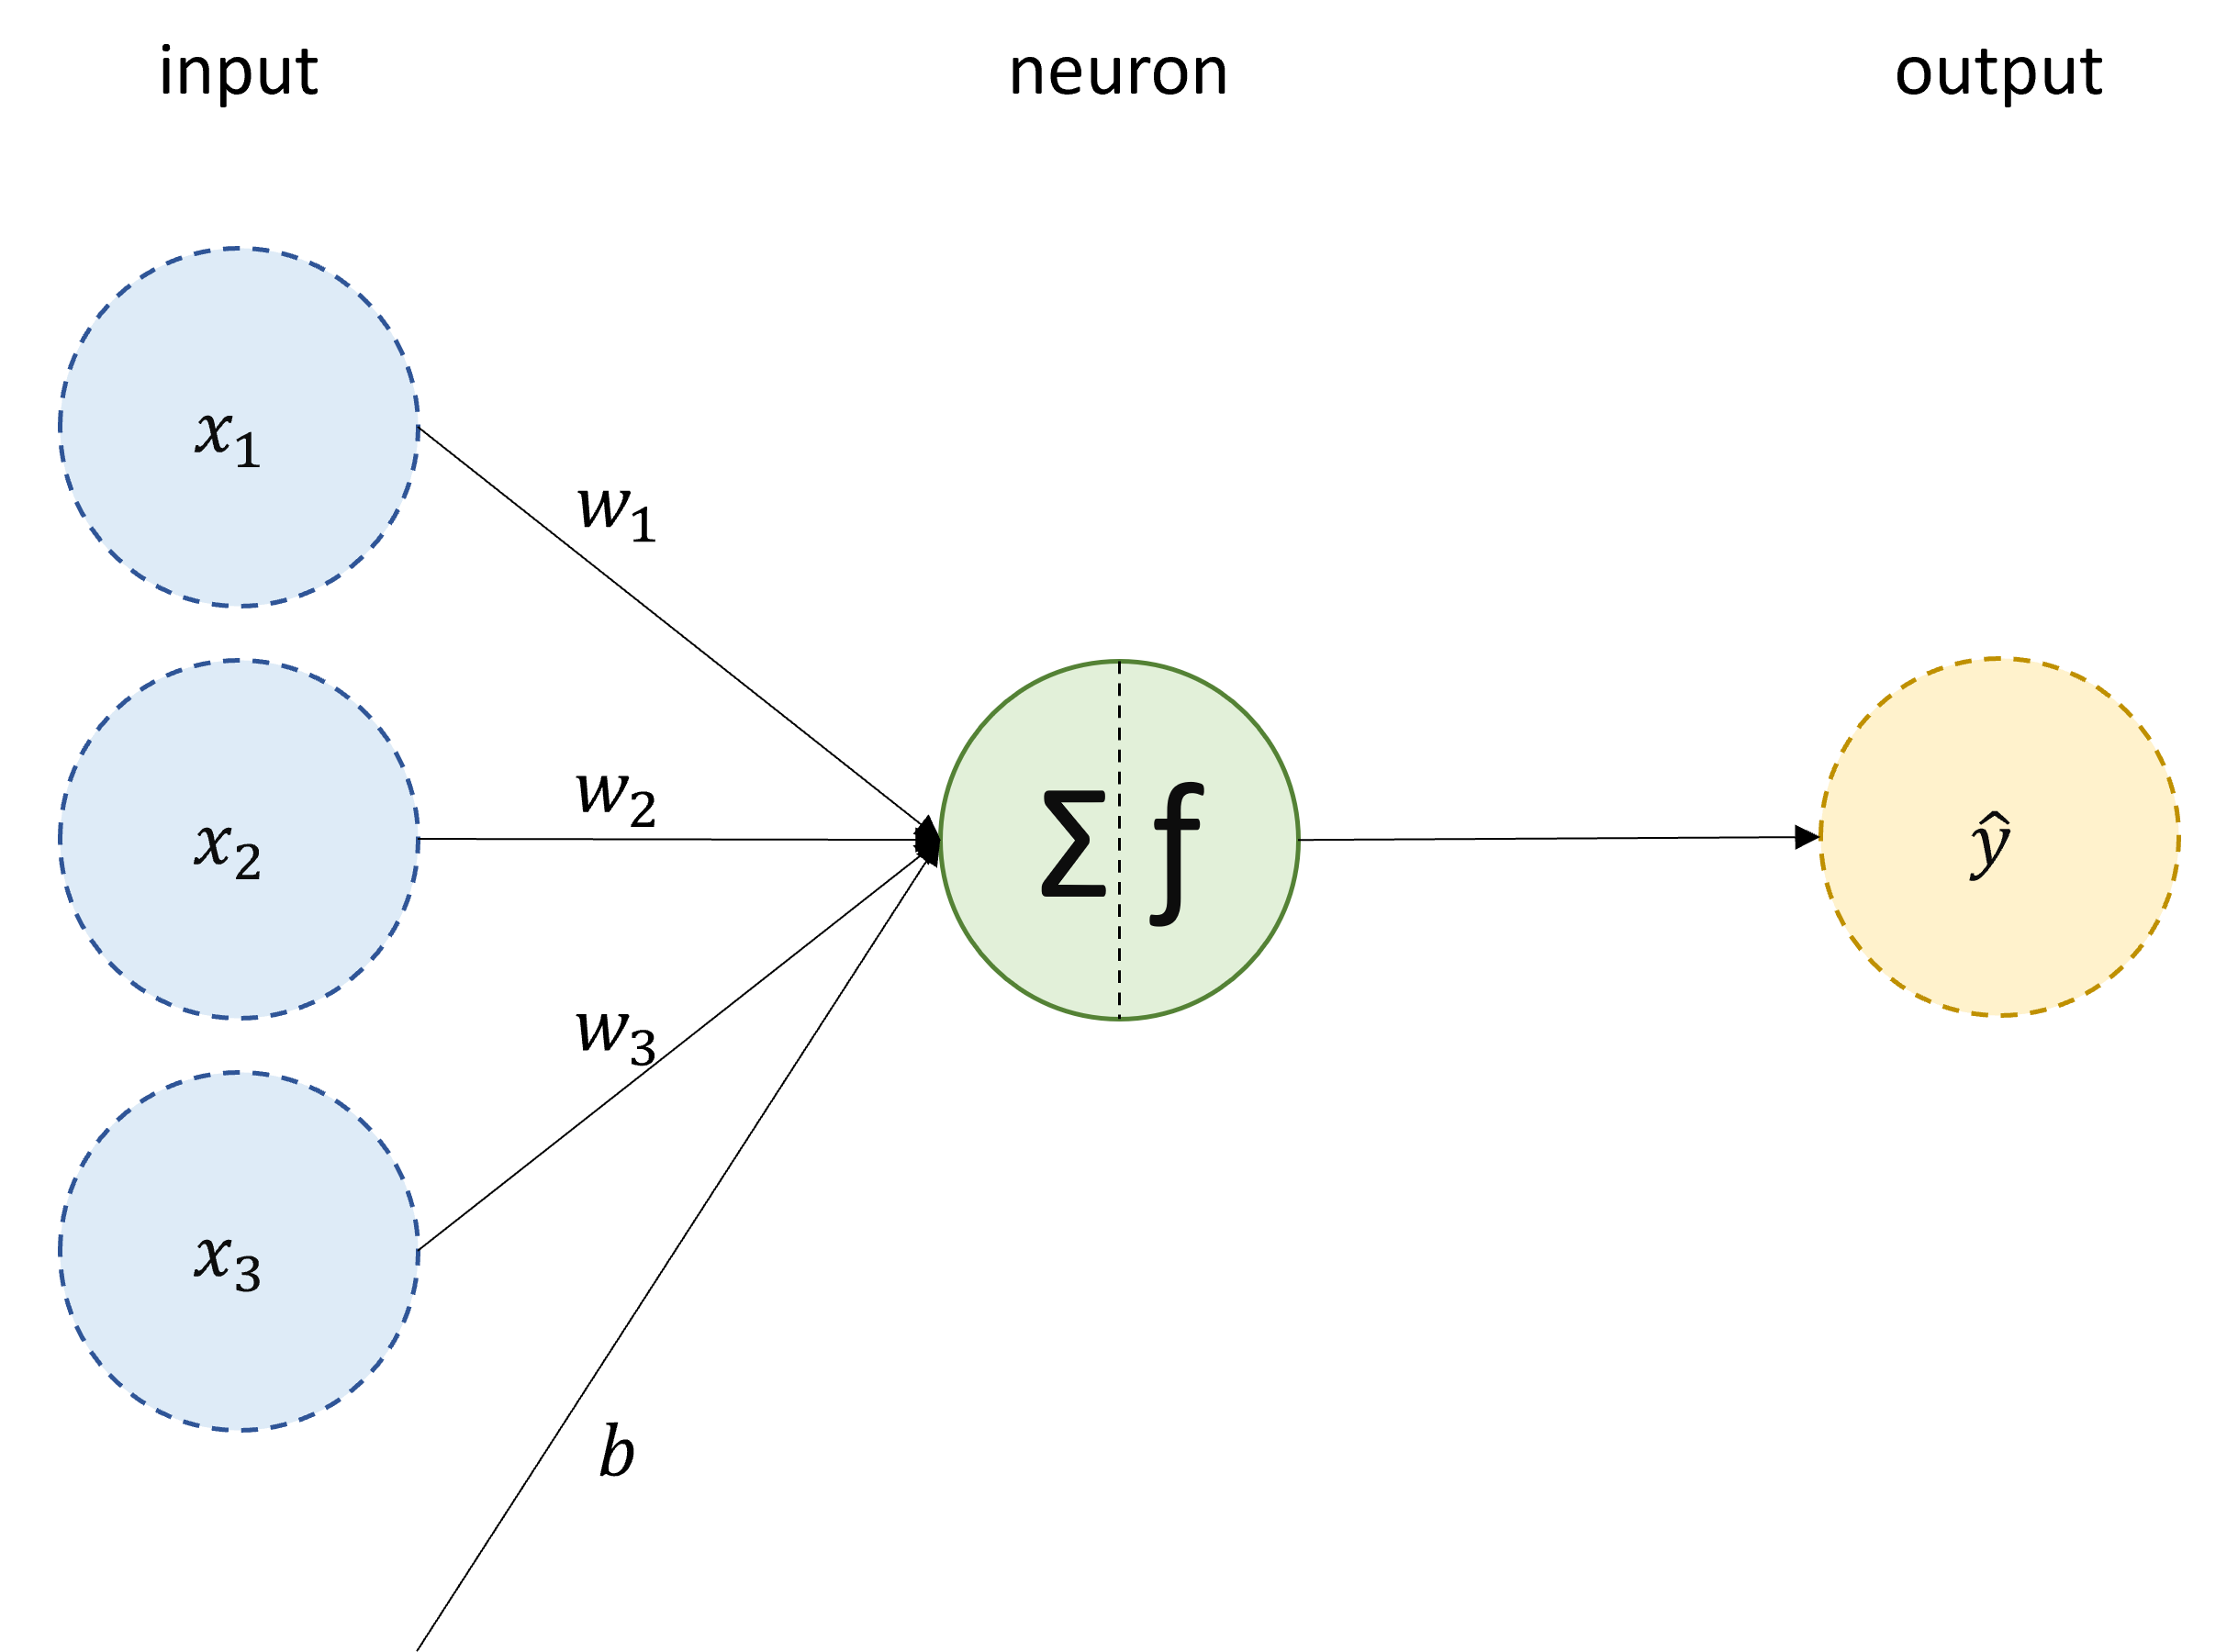
\includegraphics[width=10cm]{../images/neuron.png}
    \caption{A single neuron for binary classification}\label{fig:neuron}
    \end{center}
\end{figure}

Binary classifications usually use the sigmoid function $\sigma(z)$ as activation function to receive a fraction between 0 and 1, which can be treated as certainty. This also allows the definition of downstream threshold that favor one class to reduce type I errors.
\begin{equation}
    \sigma(z) := \frac{1}{1+e^{-z}} = \frac{e^{z}}{1+e^{z}}
\end{equation}

Classifications with more than two classes are possible by combining $K$ neurons, while $K$ is the number of classes. Thus, the weight vectors are combined in the weight matrix $\mathbf{W}$, while the biases and the outputs form the vectors $\mathbf{b}$ and $\mathbf{\hat{y}}$ respectively.
\begin{equation}
    \mathbf{W} = \begin{bmatrix}w_{1,1}&\cdots &w_{1,n}\\\vdots &\ddots &\vdots\\w_{k,1}&\cdots &w_{k,n}\end{bmatrix}\text{,}\quad\mathbf{b} = \begin{bmatrix}b_1\\\vdots \\b_k\end{bmatrix}\text{,}\quad\mathbf{\hat{y}} = \begin{bmatrix}\hat{y}_1\\\vdots \\\hat{y}_k\end{bmatrix}
\end{equation}

The softmax function is suited as activation function in such cases to produce a probability distribution as output.
\begin{equation}
    \operatorname{softmax}(\mathbf{z})_{i} := {\frac{e^{z_{i}}}{\sum_{k=1}^{K}e^{z_{k}}}}\text{ for }i=1,\dotsc ,K
\end{equation}

Figure~\ref{fig:neurons} shows such an example with four input values and three output classes.

\begin{figure}[H]
    \begin{center}
    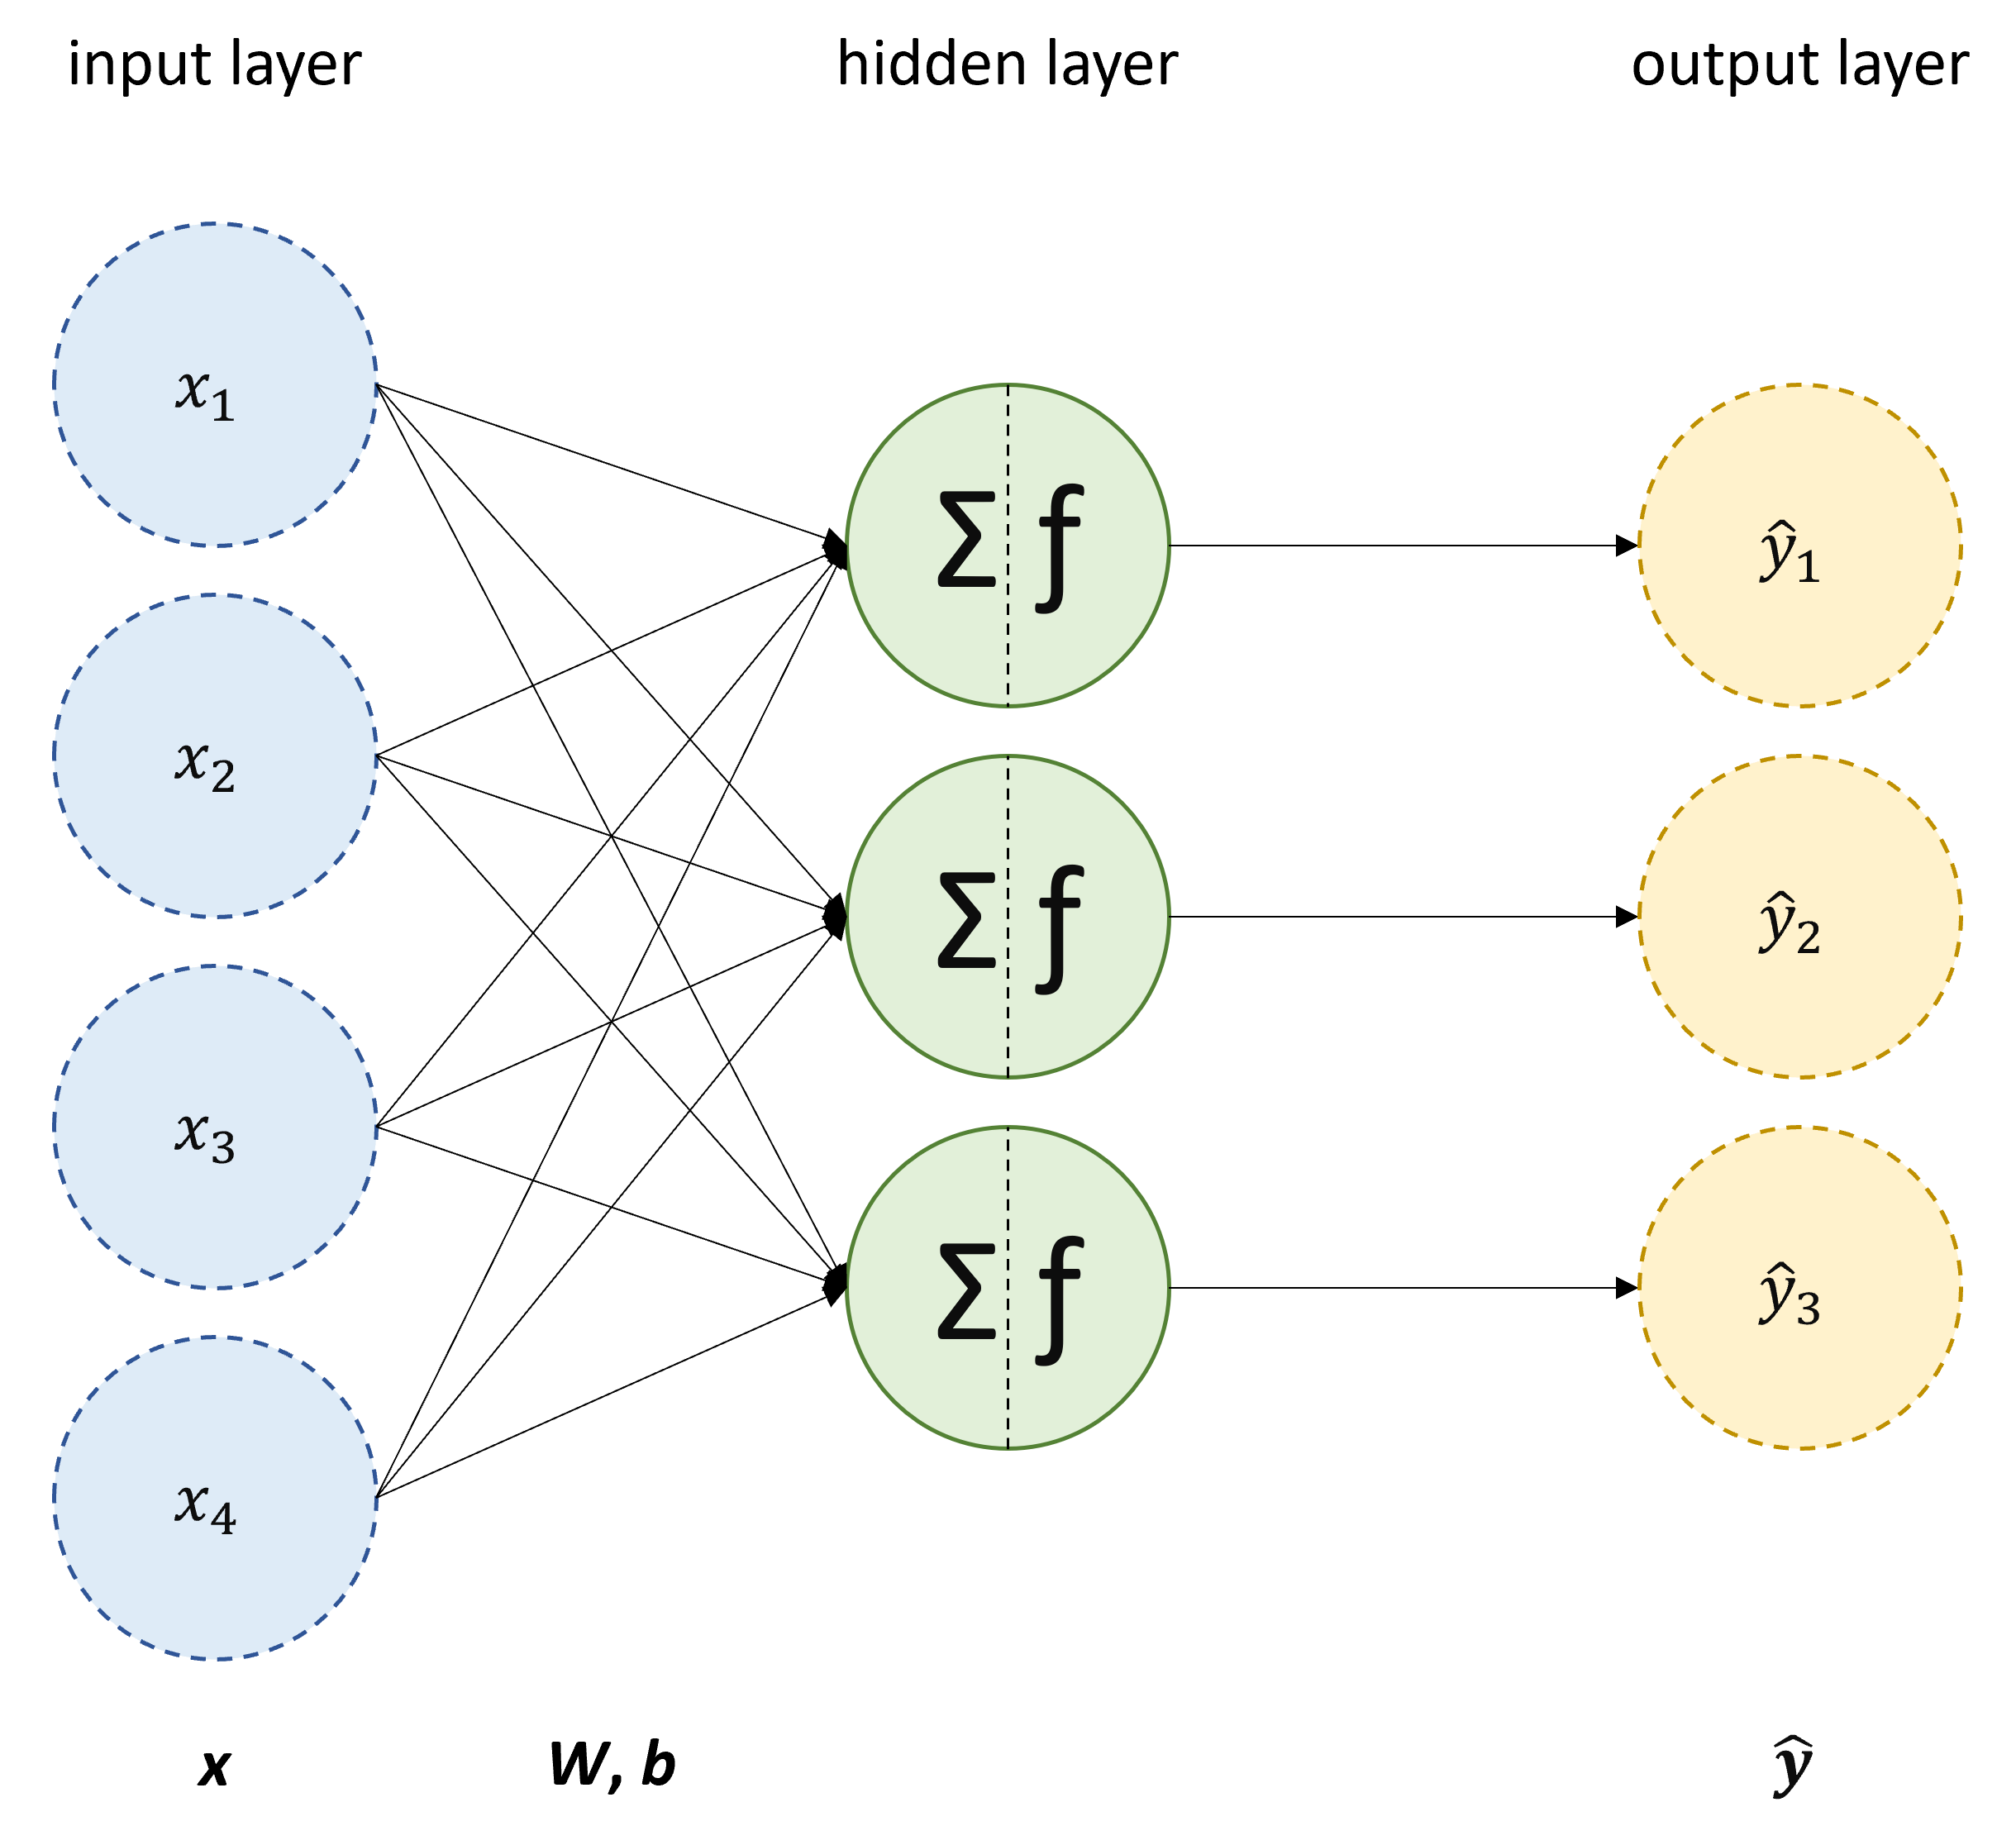
\includegraphics[width=10cm]{../images/neurons.png}
    \caption{Multiple neurons for multi class classification}\label{fig:neurons}
    \end{center}
\end{figure}

\subsection{Multilayer perceptron}
Stacking several layers of neurons leads to the \gls{mlp}. Every neuron is connected to each neuron of the previous layer making it a ``dense'' network.
$\sigma(z)$ and $\operatorname{softmax}(\mathbf{z})$ are expensive to calculate. The \gls{relu} function has a similar effect, but is much simpler and therefore better suited in all layers except the last.

\begin{equation}
\operatorname{relu}(z) := \begin{cases}z,&z>0\\0,&z\leq 0\end{cases}
\end{equation}

Figure~\ref{fig:mlp_architecture} shows the previous network with two additional hidden layers.

\begin{figure}[H]
    \begin{center}
    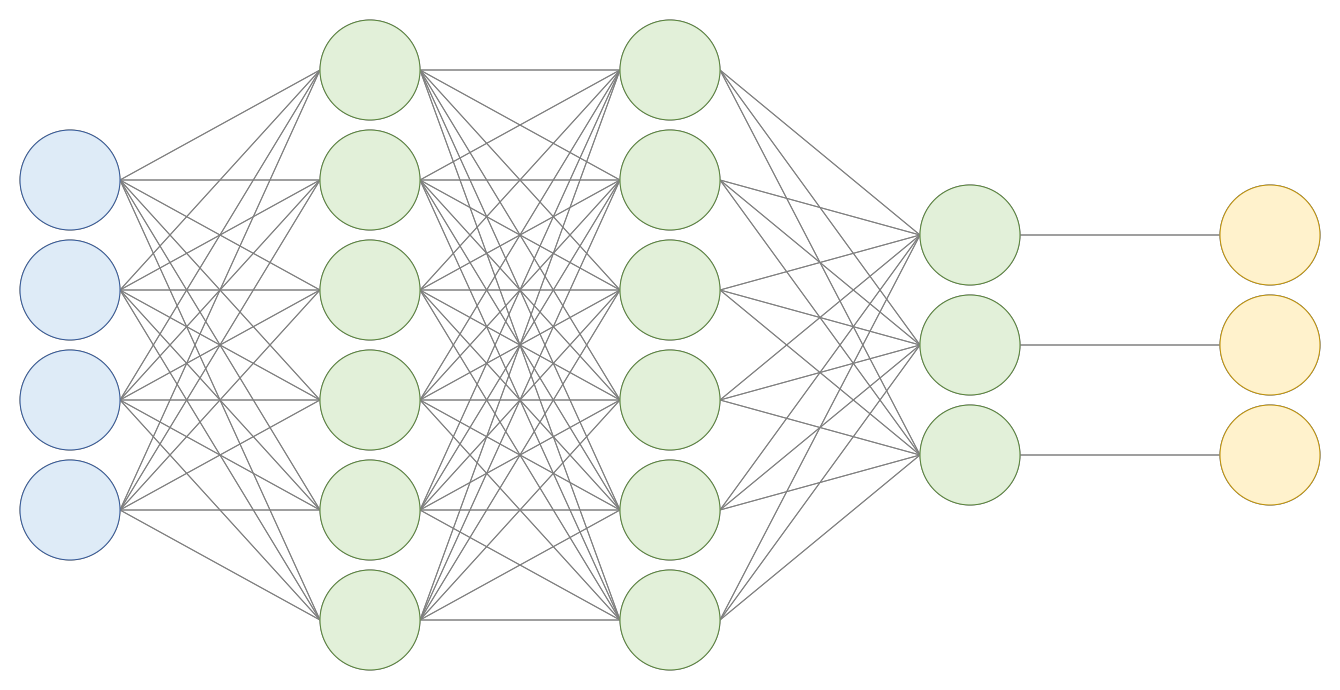
\includegraphics[width=15cm]{../images/mlp_architecture.png}
    \caption{Architecture of a basic multilayer perceptron}\label{fig:mlp_architecture}
    \end{center}
\end{figure}

% \glspl{ann} have become the de facto standard in image classification.%cite 
% The main architectures are \glspl{cnn} and the more recent \glspl{vit}.

\subsection{Convolutional neural networks}
Dense neural networks are not suited for images. Usually only the last few layers are dense to classify the extracted features. Extracting these features brings some obstacles. On one hand would a $224$ pixel high and $244$ pixel wide image already require millions of parameters per layer, which is not feasible. On the other hand should the model be resistant to small rotations and translations of the depicted object. Luckily, it is not necessary to regard all pixels in every neuron. Pixels often highly correlate with their adjacent neighbors and therefore contain redundancy.
Filters address these problems by combining pixels locally and extracting meaningful features per region \autocite{lecun1989}. The input data can be written as a two-dimensional matrix $\mathbf{G} \in \mathbb{R}^{w_g \times h_g}$, where $w_g$ and $h_g$ are the width and height of the input data. Every filter consists of a filter matrix $\mathbf{F} \in \mathbb{R}^{w_f \times h_f}$ and a bias scalar $b$, where $w_f$ and $h_f$ are analogously the width and height of that filter. During the ``convolution'' the filter is applied to the input matrix to generate the output matrix $\mathbf{O} \in \mathbb{R}^{w_o \times h_o}$.

\begin{equation}
o_{i,j} = (\mathbf{F} \ast \mathbf{G})_{i,j} = \sum_{m=1}^{w_f}\sum_{n=1}^{h_f} f_{m,n} \cdot g_{i+m, j+n} + b
\end{equation}

Depending on the values in the filter matrix $\mathbf{F}$ it is possible to carry out various operations such as finding edges or other patterns. 
Filters are usually relatively small, $3 \times 3$ pixels for example, and they use these parameters for the whole input. This ensures that the number of trainable parameters stays manageable and helps against small translations. 
Instead of producing only one output layer often multiple different filters are used on the input increasing the number of channels. 

Convolutional layers are usually alternated with pooling layers. The latter scale down the layer size and reduce the number of required neurons for classification greatly. An example of a \gls{cnn} is shown in Figure~\ref{fig:cnn_architecture}. The images is fed into the network on the left side. The convolutional layers increase the number of channels, visualized by thicker layers. The pooling layers decrease the height and width. The flattening layer concatenates all data points from the two-dimensional input batches into a one-dimensional output vector. This vector can then be used by dense layers to decrease the number of nodes to the number of classes.

\begin{figure}[H]
    \begin{center}
    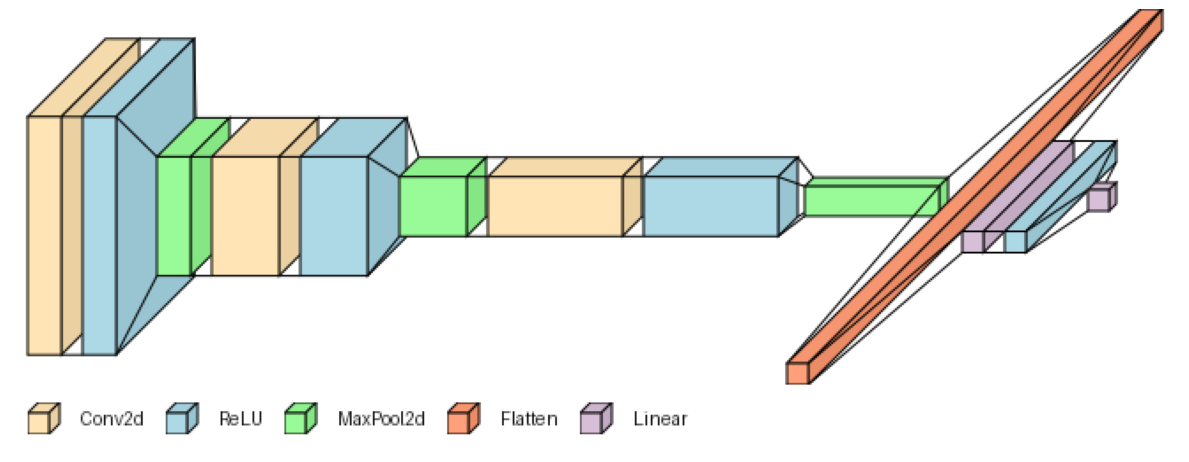
\includegraphics[width=15cm]{../images/cnn_architecture.png}
    \caption{Architecture of a basic \gls{cnn}}\label{fig:cnn_architecture}
    \end{center}
\end{figure}

\subsection{Resnet50}
Some \gls{cnn} models were able to win the ImageNet classification challenge such AlexNet \autocite{krizhevsky2012} in 2012 and \gls{vgg} \autocite{simonyan2015} in 2014. But training such deep models was laborious and reaching its limits. 

The introduction of residual connection in 2025 provided a remedy \autocite{he2015}. Residual connection copies the values of an earlier layer and adds it to a later layer. This stabilizes the training process and allows ever deeper models to be trained without vanishing gradients.
The Resnet50 architecture is one of the resulting residual neural networks, which is still widely used in image classification today. Figure~\ref{fig:resnet50_architecture} shows the structure based on the implementation from ``torchvision''. Additionally, the newly discovered batch normalization is utilized to stabilize and accelerate training \autocite{ioffe2015}.

\begin{figure}[H]
    \begin{center}
    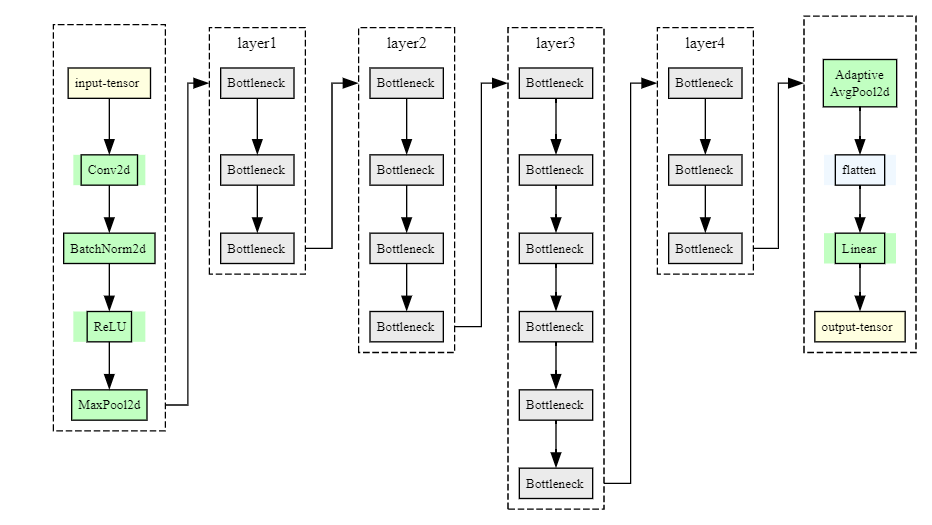
\includegraphics[width=15cm]{../images/resnet50_architecture.png}
    \caption{Architecture of Resnet50}\label{fig:resnet50_architecture}
    \end{center}
\end{figure}

Every ``bottleneck'' block contains the layers shown in Figure~\ref{fig:resnet50_architecture_bottleneck} including the mentioned residual connection.

\begin{figure}[H]
    \begin{center}
    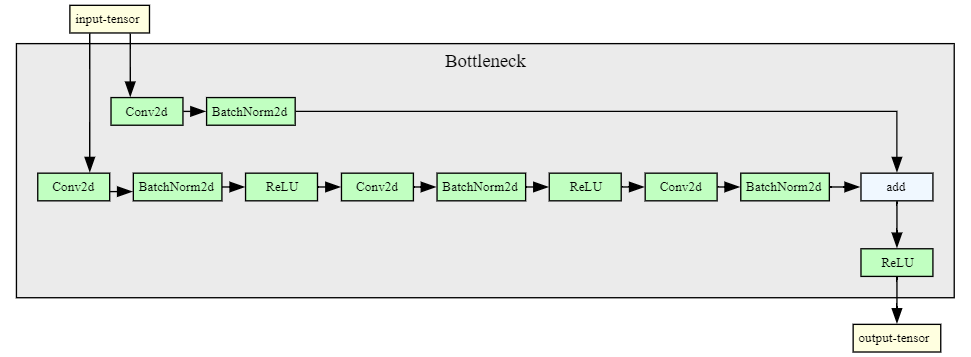
\includegraphics[width=15cm]{../images/resnet50_architecture_bottleneck.png}
    \caption{Architecture of Resnet50 bottleneck}\label{fig:resnet50_architecture_bottleneck}
    \end{center}
\end{figure}

\newpage

\subsection{Vision transformer}

\subsection{ViT-T/16}
Another major breakthrough was achieved 2017 by introducing the transformer \autocite{vaswani2017}. The transformer is able to handle context due to the concept of ``attention''. After the broad success in \gls{nlp} transformers were introduced for visual tasks as well \autocite{dosovitskiy2020}. This original \gls{vit} comes in the sizes ``base'', ``large'' and ``huge''. But further papers introduced the smaller version `tiny' \autocite{liu2021,wu2022}.

Figure~\ref{fig:vit_t16_architecture} shows the implementation of the tiny \gls{vit} in the library ``timm''. Other libraries have slightly different implementations, but this work has mainly used this version.

\begin{figure}[H]
    \begin{center}
    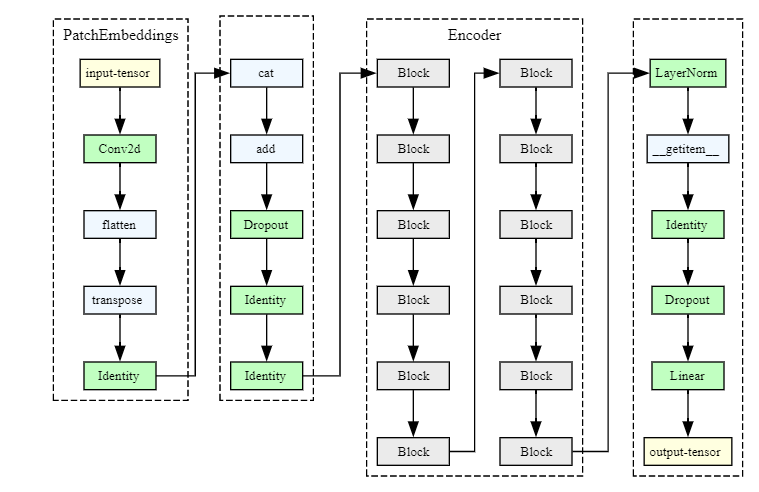
\includegraphics[width=13cm]{../images/vit_t16_architecture.png}
    \caption{Architecture of ViT-T/16}\label{fig:vit_t16_architecture}
    \end{center}
\end{figure}

Figure~\ref{fig:vit_t16_architecture_block}.

\begin{figure}[H]
    \begin{center}
    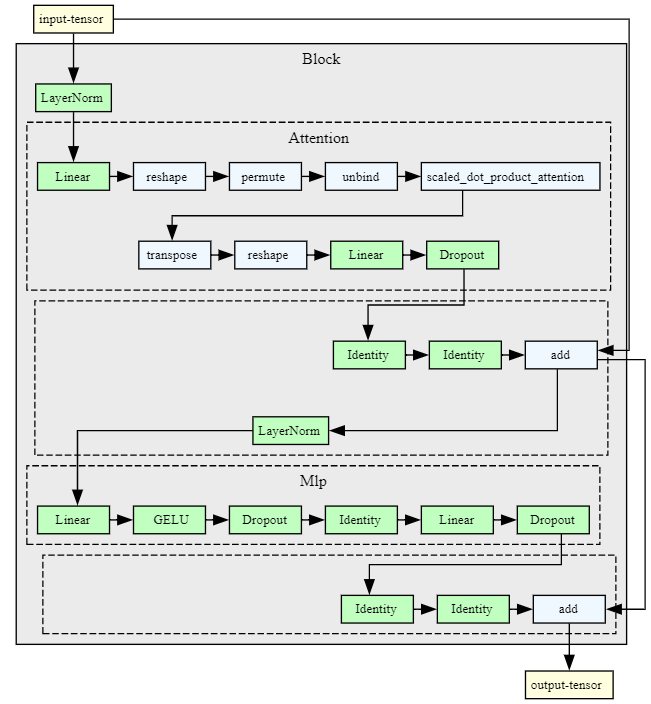
\includegraphics[width=11cm]{../images/vit_t16_architecture_block.png}
    \caption{Architecture of ViT-T/16 block}\label{fig:vit_t16_architecture_block}
    \end{center}
\end{figure}


\section{Transfer Learning}
The basic concept of transfer learning is to reuse the trained parameters for other similar tasks. It was shown, that the positive effect of transfer learning often was not achieved and sometimes even a negative effect occurred \autocite{perkins1999}. There are several approaches trying to determine the potential by measuring the relatedness of tasks \autocite{torrey2009}. In most cases the success of transfer was highly dependent on the type of \gls{ml} algorithm and even the specific architecture. There is simply no solution that fits all.

\subsection{Transfer Learning in medical imaging}
In the past years it became common practise in image classification to use the pre-trained weights such as from the ImageNet dataset and then fine-tuning on the domain specific task \autocite{russakovsky2014}. 
Among others this approach has been successfully used with \glspl{cnn} for image classification in dermatology and many other medical fields \autocite{esteva2017,lam2018,bayramoglu2016,pardamean2018,yang2018}. But some results show that ImageNet pre-training may speed up convergence early in training, but does not improve the final accuracy compared to randomly initialized models \autocite{he2018}.

Some claim that the differences between the pre-training and target data sets is considerably high and therefore the ImageNet are not suited \autocite{raghu2019}.
The main differences include the resolution, data set size and the number of classes.
\autocite{raghu2019} shows, that Resnet-50 fine-tuned on the medical datasets CheXpert and Retina does not benefit significantly from ImageNet pre-training. On the other hand \autocite{raghu2019} shows that only certain layer benefit from pre-trained weights while others should be initialized randomly. With many contradicting observations and claims but no general statement can be made, and the problem requires to be looked at specifically.


% \subsection{Linear evaluation with frozen features}
% DINO outperforms other models \autocite{truong2021}.

% \subsection{Fine-tuning}
% weight transfusion


% \subsection{Self-supervised pre-training}
% In the past years serveral approaches with \gls{ssl} pre-training was made in the field of medical image classification \autocite{zhou2019,chen2019,taleb2020,bai2019,abbet2020,sowrirajan2020}.

% Skin Lesion Analysis
% dermatology \autocite{chaves2021}

% Previous work shows better results when finetuning all layers instead of freezing earlier parts of the network \autocite{newell2020}.

% \autocite{newell2020} measure the utility 

% suggests that the utility of self-supervised pre-training comes mainly from better regularization that reduces overfitting, not better optimization
% that reduces underfitting—otherwise we should expect selfsupervision to have non-negligible utility even with large
% numbers of labeled samples

% SimCLR \autocite{chen2020}
% DINO \autocite{caron2021}
% Linear evaluation

% While there are successfull

% \autocite{kornblith2019} used \gls{cca} and \gls{cka} to compare the layers within neural networks as well as different trained models.

% \autocite{perkins1999}

% AI
% Finetuning / Transfer Learning
% Modern approaches: Lora, Adapter
% Frozen evaluation
% Utility Score

% DINO
% Teacher / Student
